\documentclass{beamer}

\usepackage[french]{babel}    % langue
\usepackage[utf8]{inputenc}   % accents
\usepackage[T1]{fontenc}      % caractères français
\usepackage{mdframed}
\usepackage{listings}

\usetheme{metropolis}

\surroundwithmdframed[
    hidealllines=true,
    backgroundcolor=orange!30,
    skipbelow=\baselineskip,
    skipabove=\baselineskip
]{align*}

\title{L'algorithme $\rho$ de Pollard}
\date{\today}
\author{Laure Bachelet, Charlotte Rance et Xavier Maso}
\institute{Master CSI, Université de Bordeaux}

\begin{document}
  \maketitle

  \begin{frame}{Plan}
    \setbeamertemplate{section in toc}[sections numbered]
    \tableofcontents[hideallsubsections]
  \end{frame}


  \section{Présentation de la méthode $\rho$}

  \begin{frame}{Problème du Logarithme Discret}
    \begin{align*}
      G = \langle g \rangle, \text{\ sous-groupe de }{\mathbb{F}_p}^*, |G| = q \text{\ premier} \\
      h \in G \implies \exists k \in \mathbb{Z} \text{\ tel que } h = g^k
    \end{align*}

    Étant donné $h$, trouver $k$ est difficile.
  \end{frame}


  \begin{frame}{Méthode de Pollard (idée générale)}
    \begin{itemize}
      \item $(x_i)_{i \ge 0}$ éléments de $G$ tels que $x_{i+1} = f(x_i)$
      \item $f: G \rightarrow G$ permet d'avoir : $\forall i, x_i = g^{a_i} \cdot h^{b_i}$ (\textbf{traçage des exposants})
    \end{itemize}


    On cherche une collision : deux indices $i$ et $j$ tels que $i \ne j$, $x_i = x_j$.

    \begin{align*}
       x_i = x_j &\implies g^{a_i} \cdot h^{b_i} = g^{a_j} \cdot h^{b_j} \\
                 &\implies h^{b_i - b_j} = g^{a_j - a_i} \\
                 &\implies (b_i - b_j) \cdot \log_g(h) \equiv a_j - a_i \text{\ mod } q
     \end{align*}
  \end{frame}


  \begin{frame}{Méthode de Pollard (algorithmes)}
    \begin{itemize}
      \item itération
        \begin{itemize}
          \item[--] "basique"
          \item[--] méthode r-adding walks
        \end{itemize}
      \item collision
        \begin{itemize}
          \item[--] le lièvre et la tortue
          \item[--] méthode des points distingués
        \end{itemize}
    \end{itemize}
  \end{frame}


  \section{Détection de collisions}

  \begin{frame}{Le lièvre et la tortue}
    $(x_i)_{i \ge 0}$ ultimement périodique~: $x_{kC+i} = x_i$, $\forall i \geq T$, $\forall k \in \mathbb{N}$
    \begin{figure}
            \center{}
            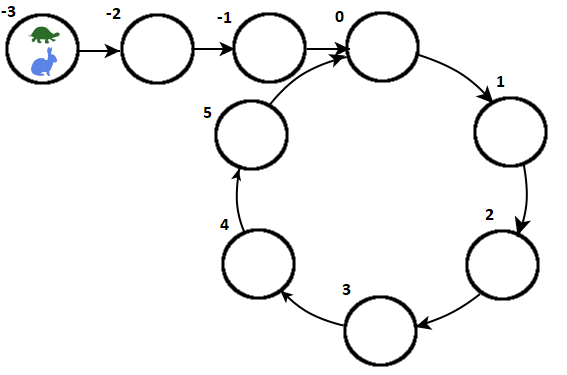
\includegraphics[scale=0.5]{../rapport/images/Floyd.png}
            \caption{Algorithme de Floyd avec $T=3$ et $C=6$}
     \end{figure}
  \end{frame}

  \begin{frame}{Méthode des points distingués}
    \begin{itemize}
        \item points distingués~: satisfont une propriété facilement vérifiable (écriture binaire se terminant par $k$ zéros)
        \item choisir $x \in G$ aléatoirement, lancer la fonction d'itération jusqu'à tomber sur un point distingué, le stocker et réitérer le procédé
        \item fin~: lorsqu'on a trouvé deux fois le même point distingué, on a alors $g^{a_i} \cdot h^{b_i} = g^{a_j} \cdot h^{b_j}$ avec $(a_i,b_i) \neq (a_j,b_j)$
    \end{itemize}
  \end{frame}


  \section{Implémentations}

  \begin{frame}{Généralités}
    en C utilisant GMP
  \end{frame}

  \begin{frame}{Tests et mesures}
  \end{frame}

  \begin{frame}{Résultats !}
    \begin{figure}
            \center{}
            \includegraphics[scale=0.4]{../rapport/images/comparaison_methodes.png}
            \caption{Nombre d'appels à la fonction d'itération selon les différentes implémentations avant la détection d'une collision en fonction de la taille de $q$}
     \end{figure}
  \end{frame}

  \begin{frame}{Améliorations}
    \begin{itemize}
      \item meilleure utilisation de GMP
        \begin{itemize}
          \item[--] \lstinline{mpz_inits, mpz_clears}
          \item[--] lecture / écriture depuis IO : \lstinline{mpz_inp_str, mpz_out_str}
        \end{itemize}
      \item amélioration des tests
        \begin{itemize}
          \item[--] tester les fonctions utilisant de l'aléa
          \item[--] utiliser un "vrai" framework de tests
        \end{itemize}
      \item différents algorithmes dans un même programme
      \item implémenter la méthode de "tag tracing"
    \end{itemize}
  \end{frame}

  \section{Conclusion}

  {\setbeamercolor{palette primary}{fg=black, bg=orange!20}
  \begin{frame}[standout]
    Questions?
  \end{frame}
  }

\end{document}
